\documentclass[11pt]{article}
\usepackage[margin=1in]{geometry}
\usepackage{amsmath,amssymb}
\usepackage{booktabs}
\usepackage{graphicx}
\usepackage{xcolor}
\usepackage{enumitem}
\setlength{\parskip}{5pt}\setlength{\parindent}{0pt}
\title{\textbf{Self-Correction Benchmark Results, Explained}\\ \large HumanEval-164, one model (gpt-5.4), three ways of checking its own work}
\author{Drew --- working notes}
\date{\today}
\begin{document}\maketitle

\section*{The one-sentence result}
When the model checks its \emph{own} wrong answer, it almost never catches it --- it accepts its own mistakes $\kappa=0.889$ (about 89\% of the time). Force it to argue \emph{against} itself (steelman) and that drops to $0.364$. Run a genuinely \emph{independent} check and it drops to $0.200$. The blind spot the paper predicts is real, and independence is what fixes it.

\begin{center}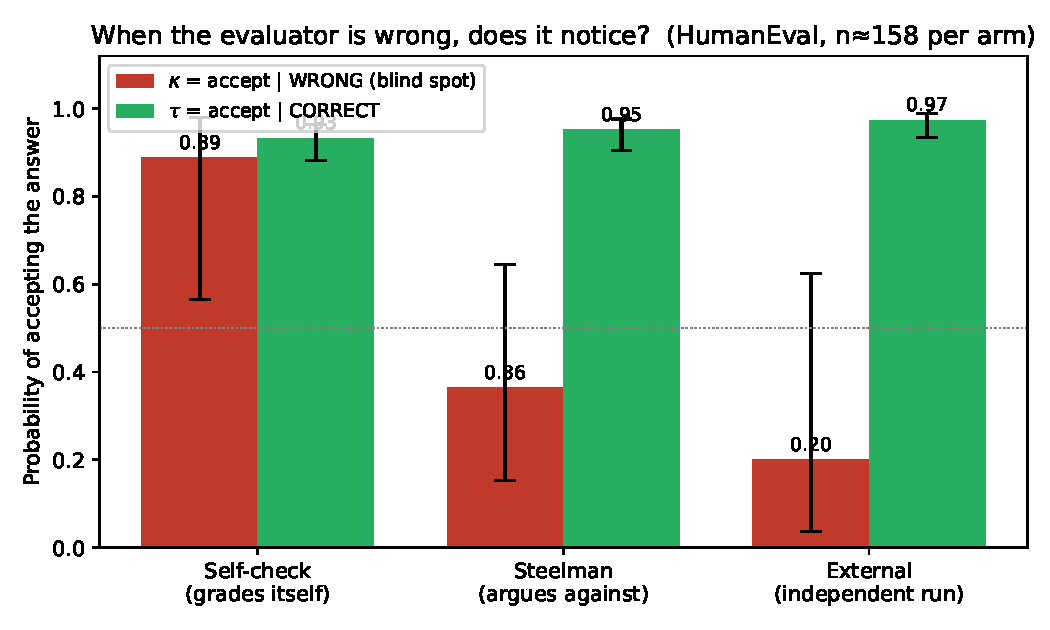
\includegraphics[width=0.95\textwidth]{fig_kappa_tau.pdf}\end{center}

\section*{The numbers}
\begin{center}
\begin{tabular}{lrrrrrr}
\toprule
arm & $n$ & $\kappa$ (accept$\mid$wrong) & $\tau$ (accept$\mid$correct) & $\Delta=\tau-\kappa$ & $\Lambda=\tau/\kappa$ & $E=\log_2\Lambda$ \\
\midrule
Self-check & 158 & 0.889 \;[0.565, 0.980] & 0.933 & 0.044 & 1.05 & 0.07 bits \\
Steelman   & 157 & 0.364 \;[0.152, 0.646] & 0.952 & 0.588 & 2.62 & 1.39 bits \\
External   & 157 & 0.200 \;[0.036, 0.624] & 0.974 & 0.774 & 4.87 & 2.28 bits \\
\bottomrule
\end{tabular}
\end{center}
Brackets are 95\% confidence intervals (explained below). $\kappa$ is the quantity the paper cares about: the probability the evaluator accepts an answer that is actually \textbf{wrong}. You want $\kappa$ \emph{low}. $\tau$ is the probability it accepts an answer that is actually correct; you want $\tau$ \emph{high}. A good evaluator has a big gap $\Delta$ between them.

\section*{What a confidence interval (CI) actually is --- the honest version}
You ran the test \emph{once} and got one number, e.g.\ $\kappa=0.889$. But that number came from a \emph{sample}. If you re-ran the whole experiment on a fresh batch of problems, you'd get a slightly different $\kappa$. The 95\% CI is the range that, \emph{if you repeated this experiment many times, would contain the true value about 95\% of the time.}

The intuition that matters for you:
\begin{itemize}[leftmargin=1.4em]
\item \textbf{Narrow CI = you measured it well. Wide CI = you barely measured it.} The width is driven almost entirely by sample size $n$.
\item CI width shrinks like $1/\sqrt{n}$. To make an interval \emph{half} as wide you need \emph{four times} the data, not twice. That is why the last bit of precision is always expensive.
\item Here the $\kappa$ intervals are wide --- [0.57, 0.98], [0.15, 0.65], [0.04, 0.62] --- because the model only got 9, 11, and 5 problems wrong in the three arms. You cannot estimate ``how often does it catch its own errors'' precisely when there are only a handful of errors to catch. \textbf{This is the main limitation and it belongs in the paper's Limitations section, stated plainly.}
\end{itemize}

\subsection*{Why ``Wilson'' intervals specifically}
The textbook CI for a proportion is $\hat p \pm 1.96\sqrt{\hat p(1-\hat p)/n}$ (the ``normal'' or Wald interval). It breaks badly when $\hat p$ is near 0 or 1, or $n$ is small --- exactly our situation ($\kappa$ near 0.9 and 0.2, $n$ of 5--11). The Wald interval can even produce impossible endpoints below 0 or above 1. The \textbf{Wilson score interval} is a small correction that stays valid for small $n$ and extreme $\hat p$, and never leaves $[0,1]$. It is the right default for paired binary data at this sample size, and it costs nothing --- same formula complexity, just better behaved.

\section*{Does the difference actually mean anything? (McNemar)}
The bars above compare \emph{separate} arms. A sharper question: on the \emph{same} problems, does switching the checker flip wrong$\to$right more often than right$\to$wrong? That is \textbf{McNemar's test}, and it uses only the ``discordant'' problems where the two arms disagree.

\begin{center}
\begin{tabular}{lccc}
\toprule
comparison & wrong$\to$right & right$\to$wrong & exact $p$ \\
\midrule
Self-check $\to$ Steelman & 11 & 5 & 0.210 \\
Self-check $\to$ External & 13 & 1 & \textbf{0.0018} \\
Steelman $\to$ External   & 10 & 4 & 0.180 \\
\bottomrule
\end{tabular}
\end{center}

Read it like this: moving from self-check to an external check, the external checker \emph{fixed} 13 problems that self-check had wrongly accepted, and only \emph{broke} 1 that self-check had right. 13-vs-1 is lopsided enough that it is very unlikely to be luck ($p=0.0018$). The other two comparisons are closer to even (11-vs-5, 10-vs-4) and are \emph{not} statistically significant --- we cannot confidently say steelman beats plain self-check on final correctness at this sample size.

\subsection*{What $p$ means, in one line}
$p$ = ``if there were really \emph{no} difference between the two checkers, how likely is a split this lopsided (or more) by pure chance?'' Small $p$ = the result would be a surprising coincidence under ``no difference,'' so we take the difference seriously. It is \emph{not} the probability that the result is real, and it says nothing about how \emph{big} the effect is --- only how surprising the pattern is under the null.

\section*{So what do we actually claim in the paper?}
\begin{enumerate}[leftmargin=1.6em]
\item The self-evaluation blind spot ($\kappa$ high) is real and large: $\approx$0.89 for a model grading its own work.
\item Independence reduces it substantially: $\kappa$ 0.89 $\to$ 0.20, and the McNemar flip (13-vs-1, $p=0.0018$) backs it.
\item We claim \emph{operationalization and direction}, not proof of the theory, and we state the wide CIs and small error-count as the limitation. That is an honest, publishable result for JACIII.
\end{enumerate}

\vspace{1em}
\hrule
\vspace{0.5em}
\small\textit{Setup: HumanEval-164, model gpt-5.4, temperature 0, single-shot. $\kappa=P(\text{accept}\mid\text{wrong})$, $\tau=P(\text{accept}\mid\text{correct})$, $\Delta=\tau-\kappa$, $\Lambda=\tau/\kappa$, $E=\log_2\Lambda$. Arms: self-check (model grades itself), steelman (model argues against itself then grades), external (independent run grades). CIs are Wilson score intervals; paired comparison is exact McNemar.}
\end{document}
